%%%%%%%%%%%%%%%%%%%%%%%%%%%%%%%%%%%%%%%%%
% Thin Sectioned Essay
% LaTeX Template
% Version 1.0 (3/8/13)
%
% This template has been downloaded from:
% http://www.LaTeXTemplates.com
%
% Original Author:
% Nicolas Diaz (nsdiaz@uc.cl) with extensive modifications by:
% Vel (vel@latextemplates.com)
%
% License:
% CC BY-NC-SA 3.0 (http://creativecommons.org/licenses/by-nc-sa/3.0/)
%
%%%%%%%%%%%%%%%%%%%%%%%%%%%%%%%%%%%%%%%%%

%----------------------------------------------------------------------------------------
%	PACKAGES AND OTHER DOCUMENT CONFIGURATIONS
%----------------------------------------------------------------------------------------

\documentclass[a4paper, 11pt]{article} % Font size (can be 10pt, 11pt or 12pt) and paper size (remove a4paper for US letter paper)

\usepackage[protrusion=true,expansion=true]{microtype}	% Better typography
\usepackage{graphicx} 		% Required for including pictures
\usepackage{wrapfig}  		% Allows in-line images
\usepackage{hyperref}		% Allows the use of hyperlinks
\usepackage{amsmath}
\usepackage{multirow}

\usepackage{mathpazo}		% Use the Palatino font
\usepackage[T1]{fontenc} 	% Required for accented characters
\usepackage[utf8]{inputenc}     % Spanish characters
\usepackage{amsmath} 		% Allows align
\usepackage{listings}		% Allows code 
\usepackage{float}		% Allows code 
\usepackage{subfig}


\lstset{basicstyle=\footnotesize\ttfamily,breaklines=true}

\linespread{1.05} % Change line spacing here, Palatino benefits from a slight increase by default

\makeatletter
\renewcommand\@biblabel[1]{\textbf{#1.}} % Change the square brackets for each bibliography item from '[1]' to '1.'
\renewcommand{\@listI}{\itemsep=0pt} % Reduce the space between items in the itemize and enumerate environments and the bibliography

\renewcommand{\maketitle}{ % Customize the title - do not edit title and author name here, see the TITLE block below
\begin{flushright} % Right align
{\LARGE\@title} % Increase the font size of the title

\vspace{50pt} % Some vertical space between the title and author name

{\large\@author} % Author name
\\\@date % Date

\vspace{40pt} % Some vertical space between the author block and abstract
\end{flushright}
}

%----------------------------------------------------------------------------------------
%	TITLE
%----------------------------------------------------------------------------------------

\title{\textbf{Árboles de decisión}}

\author{
	\textsc{Agustín Mista}\\
	\textit{Universidad Nacional de Rosario}\\
 	\textit{Introducción a la Inteligencia Artificial}
}

\date{Rosario, 2 de Mayo de 2017}

%----------------------------------------------------------------------------------------

\begin{document}

\maketitle % Print the title section

%----------------------------------------------------------------------------------------
%	ABSTRACT
%----------------------------------------------------------------------------------------

%\renewcommand{\abstractname}{Summary} % Uncomment to change the name of the abstract to something else

%\begin{abstract}
%	Cuando todo esté cocinado, voy a completar este abstract con información pertinente.
%\end{abstract}

\vspace{20pt} % Some vertical space between the abstract and first section

%----------------------------------------------------------------------------------------
%	ESSAY BODY
%----------------------------------------------------------------------------------------

\section*{Introducción}

\begin{wrapfigure}{o}{0.45\textwidth}
	\begin{center}
		\vspace{-20pt}
		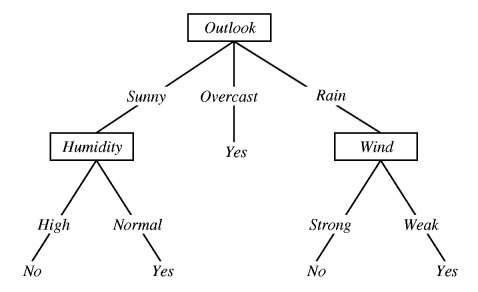
\includegraphics[width=0.4\textwidth]{play-tennis.jpg}
		\vspace{-20pt}
	\end{center}
\end{wrapfigure}

En este trabajo práctico realizamos un análisis estadístico del funcionamiento
y performance del modelo predictivo conocido como Árboles de Decisión. En
particular, analizamos los resultados obtenidos utilizando C4.5, un algoritmo
de generación de árboles de decisión desarrollado por Ross Quinlan. El mismo es
una extensión del algoritmo ID3 desarrollado anteriormente por el mismo
Quinlan. C4.5 genera árboles de decision utilizando un conjunto de datos de
entrenamiento, y basándose en el modelo de \textit{entropía de la información}.
Cada nodo del árbol generado por C4.5 es elegido como aquel que maximiza la
\textit{ganancia de información} o, en otras palabras, la diferencia de
entropía. Algunos de los aspectos que analizamos son la eficiencia de la
predicción respecto del tamaño del conjunto de entrenamiento y la resistencia
al ruido. Como conclusión de nuestro análisis, planteamos un conjunto de datos
para el cual éste modelo predictivo resulta completamente inadecuado. 

\pagebreak

%------------------------------------------------

\section*{Apartado 4}  \textit{Genere tres conjuntos de datos de entrenamiento
correspondientes al problema de las espirales anidadas de la práctica 0, uno de
longitud 150, otro de 600 y un tercero de 3000. Genere un conjunto de test de
longitud 10000. A partir de cada uno de los conjuntos de entrenamiento,
desarrolle el árbol de decisión correspondiente y grafique las predicciones
sobre el conjunto de test. Comente los resultados.}\\

La siguiente figura muestra los distintos conjuntos de entrenamiento utilizados
para generar árboles de decisión que clasifican valores en el problema de las
espirales anidadas. Cada par de figuras muestra el conjunto de entrenamiento y
su respectiva predicción para nuestro universo de 10000 elementos. Se aprecia
que, claramente, el tamaño del conjunto de entrenamiento es un factor
fundamental a la hora de generar árboles de decisión. Las predicciones de
aquellos árboles entrenados con 150, y 600 elementos resultan absolutamente
inadecuadas. La predicción del árbol de decisión entrenado con 3000 elementos
llega a predecir de manera aceptable los valores de nuestro universo, aunque se
siguen observando límites \textit{escalonados} entre ambos espirales. Ésto
último podría deberse a priori a la discretización de las variables continuas
efectuadas por C4.5 (para obtener límites más suaves entre ambas espirales se
debería utilizar algún método más sofisticado que no discretize las reglas de
decisión).

\begin{figure}[H]
\captionsetup[subfigure]{labelformat=empty}
  \centering
  \caption*{\textbf{Entrenamiento con n=150.}}
  \subfloat[][Entrenamiento]{\includegraphics[width=0.5\textwidth]{{spiral150.data}.png}}
  \subfloat[][Predicción]{\includegraphics[width=0.5\textwidth]{{spiral150.prediction}.png}}
\end{figure}

%------------------------------------------------

\begin{figure}[H]
\captionsetup[subfigure]{labelformat=empty}
  \centering
  \caption*{\textbf{Entrenamiento con n=600.}}
  \subfloat[][Entrenamiento]{\includegraphics[width=0.5\textwidth]{{spiral600.data}.png}}
  \subfloat[][Predicción]{\includegraphics[width=0.5\textwidth]{{spiral600.prediction}.png}}

  \centering
  \caption*{\textbf{Entrenamiento con n=3000.}}
  \subfloat[][Entrenamiento]{\includegraphics[width=0.5\textwidth]{{spiral3000.data}.png}}
  \subfloat[][Predicción]{\includegraphics[width=0.5\textwidth]{{spiral3000.prediction}.png}}
\end{figure}


\section*{Apartado 5.} 
\textbf{Dependencia con la longitud del conjunto de entrenamiento.
Sobreajuste y prunning:}\\ 
\textit{Genere datasets usando el programa diagonal y paralelo, con C = 0.78 y
d = 2. Genere un único conjunto de test con n = 10000.  Genere 20 conjuntos de
entrenamiento para cada uno de los siguientes valores de n: 100, 200, 300, 500,
1000, 5000.  Corra el c4.5 sobre estos datos, y con los resultados obtenidos
genere dos pares de gráficas: en el primer par, usando los resultados "before
prunning", la primer gráfica tiene el training error y test error
(porcentuales), y la segunda la cantidad de nodos en el árbol, todos como
función de la longitud del conjunto de entrenamiento (utilice siempre el
promedio de los 20 conjuntos de cada longitud dada). En el segundo par de
gráficas repita el proceso para los resultados "after prunning".  Finalmente,
repita todo el procedimiento completo usando como generador de datos el
paralelo. Incluya los resultados correspondientes en las mismas graficas del
diagonal. Discuta brevemente los resultados.}\\

El siguiente par de figuras muestra, por un lado, el error porcentual en la
predicción de los árboles de decisión generados para los problemas diagonal y
paralelo, y por el otro los tamaños de los árboles resultantes antes y despues
de ser podados, usando conjuntos de entrenamiento de 100, 200, 300, 500, 1000,
y 5000 elementos en ambos casos.

En el caso del error porcentual, puede apreciarse que el problema diagonal
obtiene predicciónes en el conjunto de entrenamiento muy similares al del
problema paralelo para cada tamaño del conjunto de entrenamiento usado. Sin
embargo, cuando se analizan las predicciones en el conjunto de test, se aprecia
que el árbol de decisión generado para el problema paralelo tiene una precisión
de entre $\sim1\%$ y un $\sim2\%$ mayor que el correspondiente al problema
diagonal, para cada tamaño del conjunto de entrenamiento.

Si analizamos ambos problemas vs. el tamaño del conjunto de entrenamiento, se
aprecia que la precisión de las predicciones aumenta dramáticamente a medida
que se amplía el tamaño del conjunto de entrenamiento para tamaños menores a
1000 elementos, pero que luego tiende a reducirse la mejoría al variar entre
conjuntos de entrenamiento mucho más poblados ($\sim13\%$ de mejoría entre 100
y 500 vs. $\sim2\%$ de mejoría entre 1000 y 5000). Esto sugeriría que la mayor
precisión se alcanza para valores entre 1000 y 5000 elementos, sin llegar a
sobreajustar el árbol de decisión generado.

A la hora de analizar el tamaño del árbol de decisión generado para ambos
problemas antes y después del podado del mismo, podemos notar que el tamaño del
árbol para el problema diagonal tiene a crecer continuamente a medida que se
aumenta el tamaño del conjunto de entrenamiento, mientras que para el caso del
problema paralelo el árbol generado tiene un tamaño prácticamente constante,
incluso antes de ser podado. Esta diferencia podría deberse a la naturaleza más
predecible del problema paralelo, en el cual podría clasificarse un valor de
manera aceptable teniendo en cuenta únicamente su valor sobre la componente X. 

\begin{figure}[H]
\captionsetup[subfigure]{labelformat=empty}
  \centering
  \caption*{\textbf{Error porcentual vs. tamaño del conjunto de entrenamiento.}}
  \subfloat[][Before prunning]{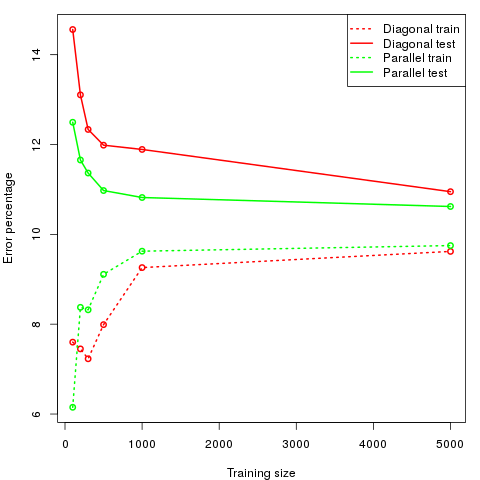
\includegraphics[width=0.5\textwidth]{sized_error_before_prunning.png}}
  \subfloat[][After prunning]{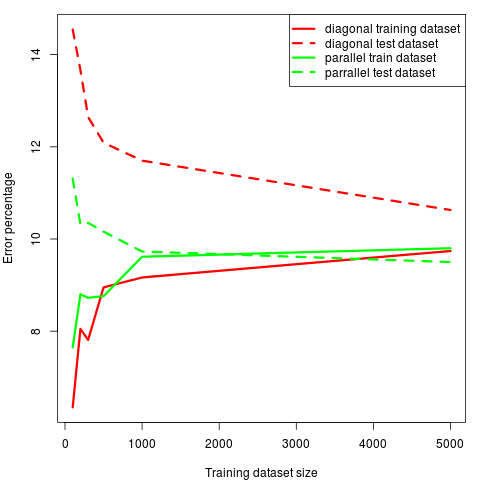
\includegraphics[width=0.5\textwidth]{sized_error_after_prunning.png}}
\end{figure}

%------------------------------------------------

\begin{figure}[H]
\captionsetup[subfigure]{labelformat=empty}
  \centering
  \caption*{\textbf{Tamaño del árbol de decisión vs. tamaño del conjunto de entrenamiento.}}
  \subfloat[][Before prunning]{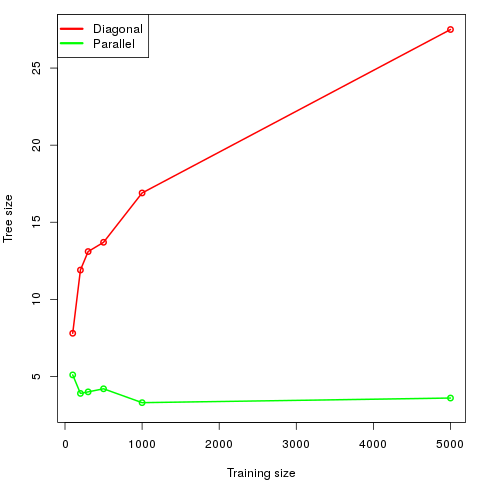
\includegraphics[width=0.5\textwidth]{sized_size_before_prunning.png}}
  \subfloat[][After prunning]{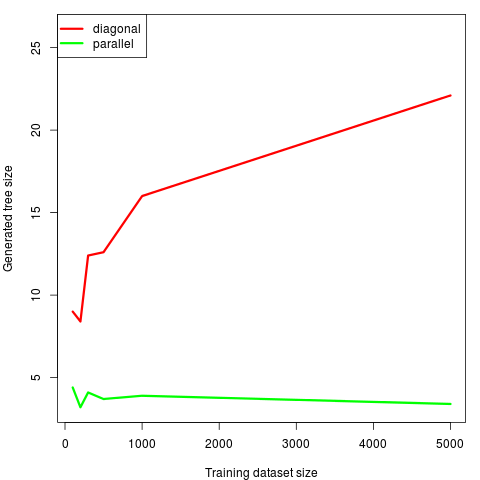
\includegraphics[width=0.5\textwidth]{sized_size_after_prunning.png}}
\end{figure}


\section*{Apartado 6}  
\textbf{Resistencia al ruido:} \textit{Genere datasets con d = 5, n = 250 para
el conjunto de entrenamiento y n = 10000 para el de test, variando el valor de
C (overlapping de las clases) de 0.5 a 2.5 con incrementos de 0.5. Como en el
punto 5, para cada valor dado de C cree 20 conjuntos distintos de
entrenamiento, pero uno solo de test.  Genere una gráfica del test-error
porcentual en función de C para el problema paralelo y el diagonal (sólo los
promedios de los 20 conjuntos para cada valor de C, los resultados de los dos
problemas en la misma gráfica). También incluya en la gráfica los valores
mínimos que se piden en el opcional 6.1.  Discuta los resultados.\\
\textbf{Opcional: }Puede calcular para cada valor de C cuál es el mínimo error
que se puede conseguir? Cómo se comparan dichos valores con los obtenidos con
el c4.5?  Obtenga una curva de error mínimo y agréguela a la gráfica anterior.
Hay varias maneras de hacerlo. Una simple es imaginando cual es el clasificador
ideal o de mínimo error para este problema (a ese clasificador se lo llama
"clasificador de Bayes") y midiendo directamente sobre un conjunto de test
grande (10000 puntos para d=5) cuántos puntos son mal clasificados por ese
clasificador ideal.}\\

El siguiente par de figuras muestra el error porcentual en la predicción vs. la
dispersión de los valores C para los problemas diagonal y paralelo tanto antes
como despues de podar los árboles generados.

Para obtener una estimación del mínimo error posible, se implementaron
clasificadores óptimos para cada problema, que determinan la clase de un punto
en el espacio basándose  en la distancia euclídea del mismo al centro de la
nube de puntos (y por ende la clase) más cercana.

En ambas gráficas se advierte algo que suena lógico, a mayor dispersión, se
torna más difícil clasificar un punto, ya que las nubes de puntos
correspondientes a cada clase comienzan a solaparse. Por otro lado, se observa
que el problema paralelo tiende a obtener mejores resultados para cada valor de
dispersión que el problema diagonal, acercándose mucho a ser un clasificador
óptimo. 

\begin{figure}[H]
\captionsetup[subfigure]{labelformat=empty}
  \centering
  \caption*{\textbf{Error porcentual vs. dispersión.}}
  \subfloat[][Before prunning]{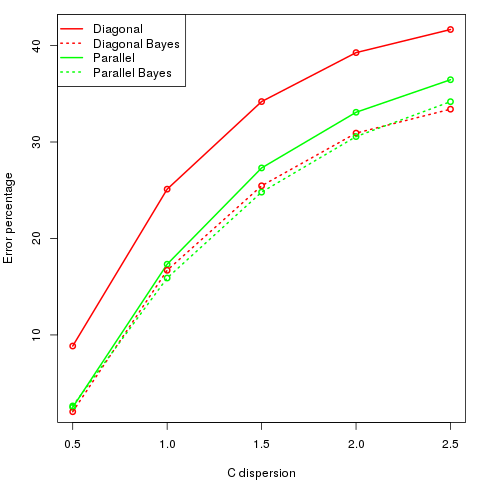
\includegraphics[width=0.5\textwidth]{noise_error_before_prunning.png}}
  \subfloat[][After prunning]{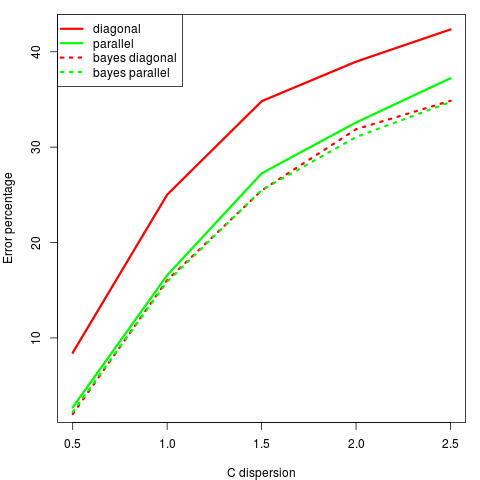
\includegraphics[width=0.5\textwidth]{noise_error_after_prunning.png}}
\end{figure}

%------------------------------------------------

\section*{Apartado 7}
\textbf{Dimensionalidad: } \textit{Genere datasets con C = 0.78, n = 250 para
el conjunto de entrenamiento y n = 10000 para el de test, variando esta vez el
valor de d según la siguiente lista: 2, 4, 8, 16, 32. Para cada valor de d cree
20 conjuntos distintos de entrenamiento, y uno solo de test. Genere una gráfica
del train y test error porcentual en función de d para el problema paralelo y
el diagonal (todos en la misma gráfica). Discuta los resultados.}\\

El siguiente par de gráficas se muestran los error porcentuales en la
predicción sobre el conjunto de entrenamiento y sobre el conjunto de test vs.
la cantidad de variables independientes en los datos.

Se puede apreciar que en los conjuntos de entrenamiento, a mayor cantidad de
variables independientes, el error disminuye. Pero dado que en el conjunto de
test se produce el efecto contrario, se puede suponer que los árboles de
decisión generados comienzan a sobreajustarse a los valores de entrenamiento,
volviéndose cada vez más imprecisos a la hora de predecir nuestro universo.

Por otro lado, el error porcentual en la predicción sobre el conjunto de test
crece de distinta manera para los problemas diagonal y paralelo a medida que se
aumenta la cantidad de variables. Se puede notar que el problema diagonal se
vuelve impresizo más rápidamente, lo cual podría deberse a que nuestros
generadores poseen distinta dispersión de datos dependiendo de la
dimensionalidad elegida. El generador de datos para el problema diagonal posee
una dispersión proporcional al valor d, mientras que en el generador de datos
para el problema paralelo la dispersión se mantiene constante.

\begin{figure}[H]
\captionsetup[subfigure]{labelformat=empty}
  \centering
  \caption*{\textbf{Error porcentual vs. dimensionalidad.}}
  \subfloat[][Before prunning]{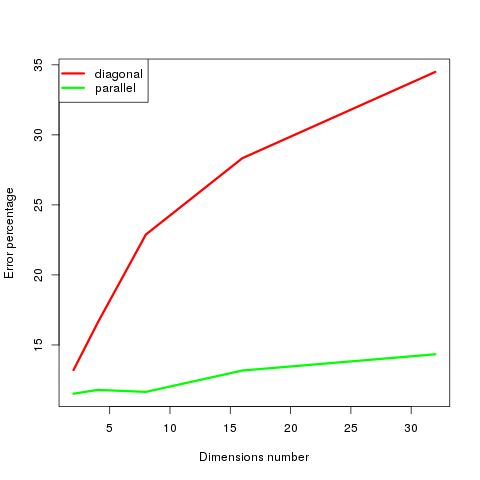
\includegraphics[width=0.5\textwidth]{dimmed_error_before_prunning.png}}
  \subfloat[][After prunning]{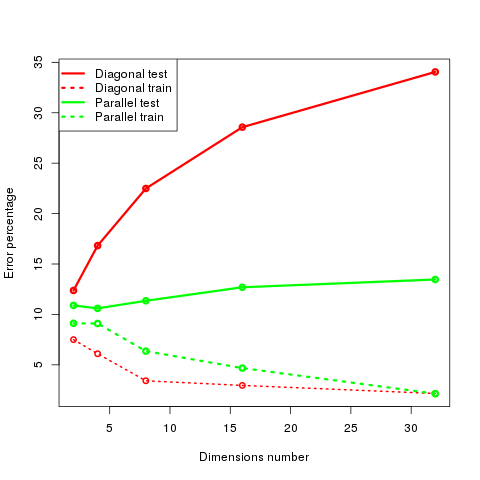
\includegraphics[width=0.5\textwidth]{dimmed_error_after_prunning.png}}
\end{figure}

%------------------------------------------------

\section*{Apartado 8} 
\textit{Baje de la página de datasets los archivos correspondientes al problema
XOR. Grafique las clases. Observando el problema, indique cuál es el árbol más
simple que clasifica correctamente todos los puntos. Aplique ahora el c4.5 a
este problema, y explique el resultado obtenido.}\\

\begin{figure}[H]
\captionsetup[subfigure]{labelformat=empty}
  \centering
  \caption*{\textbf{XOR dataset}}
  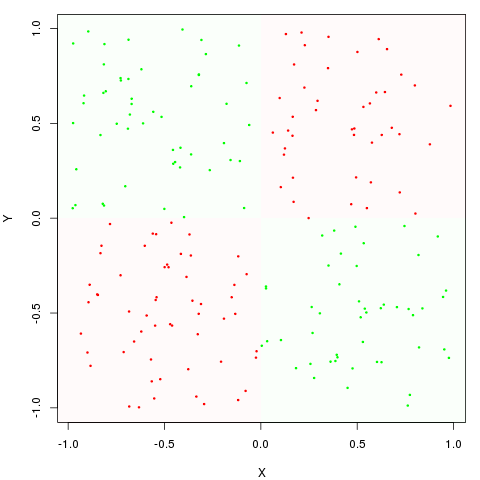
\includegraphics[width=0.7\textwidth]{xor_classes.png}
\end{figure}

El problema XOR representa un desafío para los algoritmos de clasificación
convencionales. En el caso de C4.5, el algoritmo plantea dos particiones de los
valores, cada una correspondiendo a uno de los ejes del plano. Dada la
naturaleza de los datos, ninguna de las anteriores permite obtener una ganancia
de información no nula, ya que cada partición contiene la misma cantidad de
valores de cada clase. Por consecuente, el algoritmo se detiene clasificando a
todos los valores dentro de una misma clase (con una consiguiente tasa de error
del 50\%):\\

\begin{lstlisting}[language=Bash, xleftmargin = 2cm]
$ ./c4.5 -f datasets/xor/xor -v 2

...

Read 200 cases (6 attributes) from datasets/xor/xor.data

200 items, total weight 200.0
	Att x	no gain
	Att y	no gain
	no sensible splits  200.0/100.0

Decision Tree:
 0 (200.0/100.0)
\end{lstlisting}

Por otro lado, puede escribirse un árbol de decisión para el problema XOR muy
sencillo, simplemente considerando en qué cuadrante se encuentra el punto a
clasificar:\\

\begin{lstlisting}[language=Python, xleftmargin = 2cm]
x <= 0 :
|   y <= 0 : 0
|   y > 0  : 1
x > 0 :
|   y <= 0 : 1
|   y < 0  : 0
\end{lstlisting}


\end{document}
